\documentclass[11pt]{article}
\usepackage{geometry}
\usepackage[colorlinks]{hyperref}
\usepackage{graphicx}
\usepackage{mathpazo}
\usepackage{epstopdf}
\usepackage[parfill]{parskip}
\usepackage{fancyvrb}

\makeatletter
\let \@sverbatim \@verbatim
\def \@verbatim {\@sverbatim \verbatimplus}
{\catcode`'=13 \gdef \verbatimplus{\catcode`'=13 \chardef '=13 }} 
\makeatother

\newcommand{\R}{\textsf{R}}

\begin{document}

\textbf{CVEN 4333, Spring 2010, Assignment \#7, Due Friday March 5 at 5:00 in Cameron Bracken's mailbox. No late papers accepted.}

Please include the \textsf{R} script you create with this assignment.

\begin{enumerate}

%%%%%%%%%%%%%%%%%%%%%%%%%%%%%%%
%%%%%%%%%%%%%%%%%%%%%%%%%%%%%%%
\item Book problem 7.1
\item Book problem 7.3
\item Book problem 7.6
\item Book problem 7.11

\item Below are three figures pertaining to the hydrology of Boulder creek. First look at the overall picture of water in the west (Figure 1)
\begin{enumerate}
\item Briefly describe the state of snowpack in the west, particulalry in Colorado. What implications does this have for spring runoff and streamflow?


\item How many snotel sites are there across the west? Discuss the implications of this

\item What are snotel sites? - do a search

\item compare the Boulder creek map of snotel sites. How many do we rely on the assess our water supply? What are the implications of this?


\item Now look at the map of stream flowguages. Why are there more of
     these? Does it look well covered?

\item How big in sq kilometers is the drainage area into Boulder creek? Look it up or estimate.
\end{enumerate}

\item Random numbers have important applications in hydrology.  Many hydrologic parameters are typically have randomness associated with them.  Assume that we know a hydrologic parameter $p$ is distributed normally with a mean 0 and standard deviation 1 (a standard normal variate). In \textsf{R} we can simulate standard normal random numbers with the \texttt{rnorm()} function.

\begin{enumerate}
\item Generate a data frame with 50 columns containing 5 simulations of $p$. Plot each simulation as a boxplot with a horizontal line representing the population mean (at zero). Try it a few times on your own to convince yourself that the simulations will change each time. 
\begin{verbatim}
x <- as.data.frame(matrix(rnorm(50*5),ncol=50))
names(x) <- 1:50
boxplot(x,cex=.5,ylim=c(-3,3))
\end{verbatim}

Explain the high degree of variability.
\item Repeat part (a) with 50 and with 500 samples in each column.  Explain the difference between these plots. 
\item Along these same lines create histograms of sample sizes 5, 50, 500 and 5000. Plot all four in one figure using the layout command.  Superimpose the theoretical normal distribution on top of these histograms. Explain what you observe.  Here is an example:

\begin{verbatim}
x <- seq(-3,3,,1000)
p.theory <- dnorm(x)
p.sample <- rnorm(25)
hist(p.sample,freq=F,xlim=c(-3,3))
lines(x,p.theory)
\end{verbatim}


\end{enumerate}
\end{enumerate}

\begin{figure}[htbp] %  figure placement: here, top, bottom, or page
   \centering
   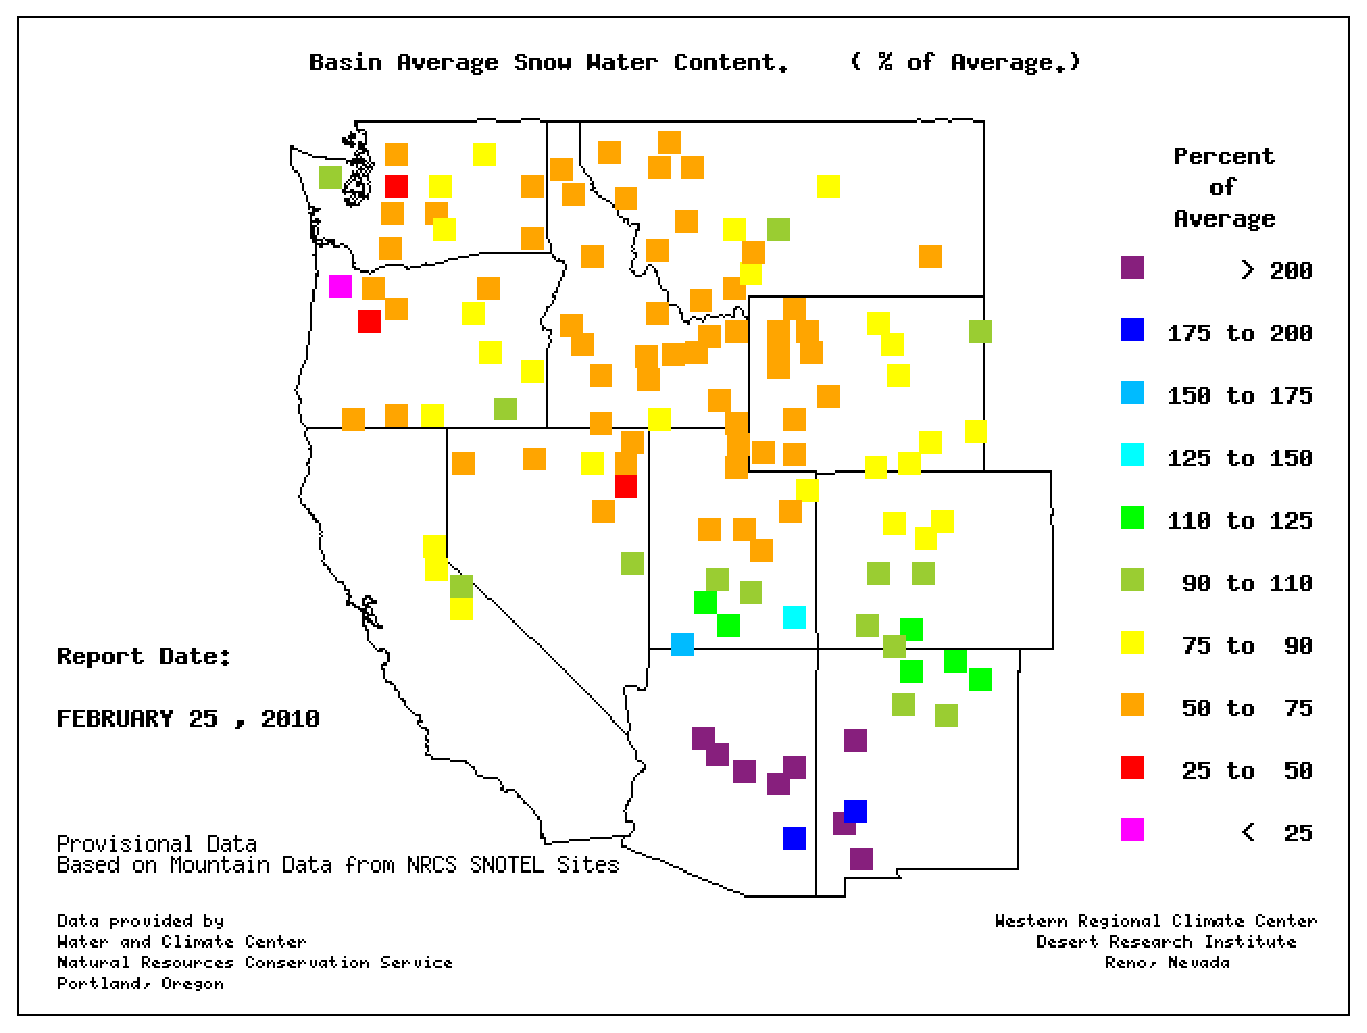
\includegraphics[width=\textwidth]{snotswe.eps} 
   \caption{SNOTEL - River Basin Snow Water Content. (source: \url{http://www.wrcc.dri.edu/snotelanom/basinswe.html})}
\end{figure}

\begin{figure}[htbp] %  figure placement: here, top, bottom, or page
   \centering
   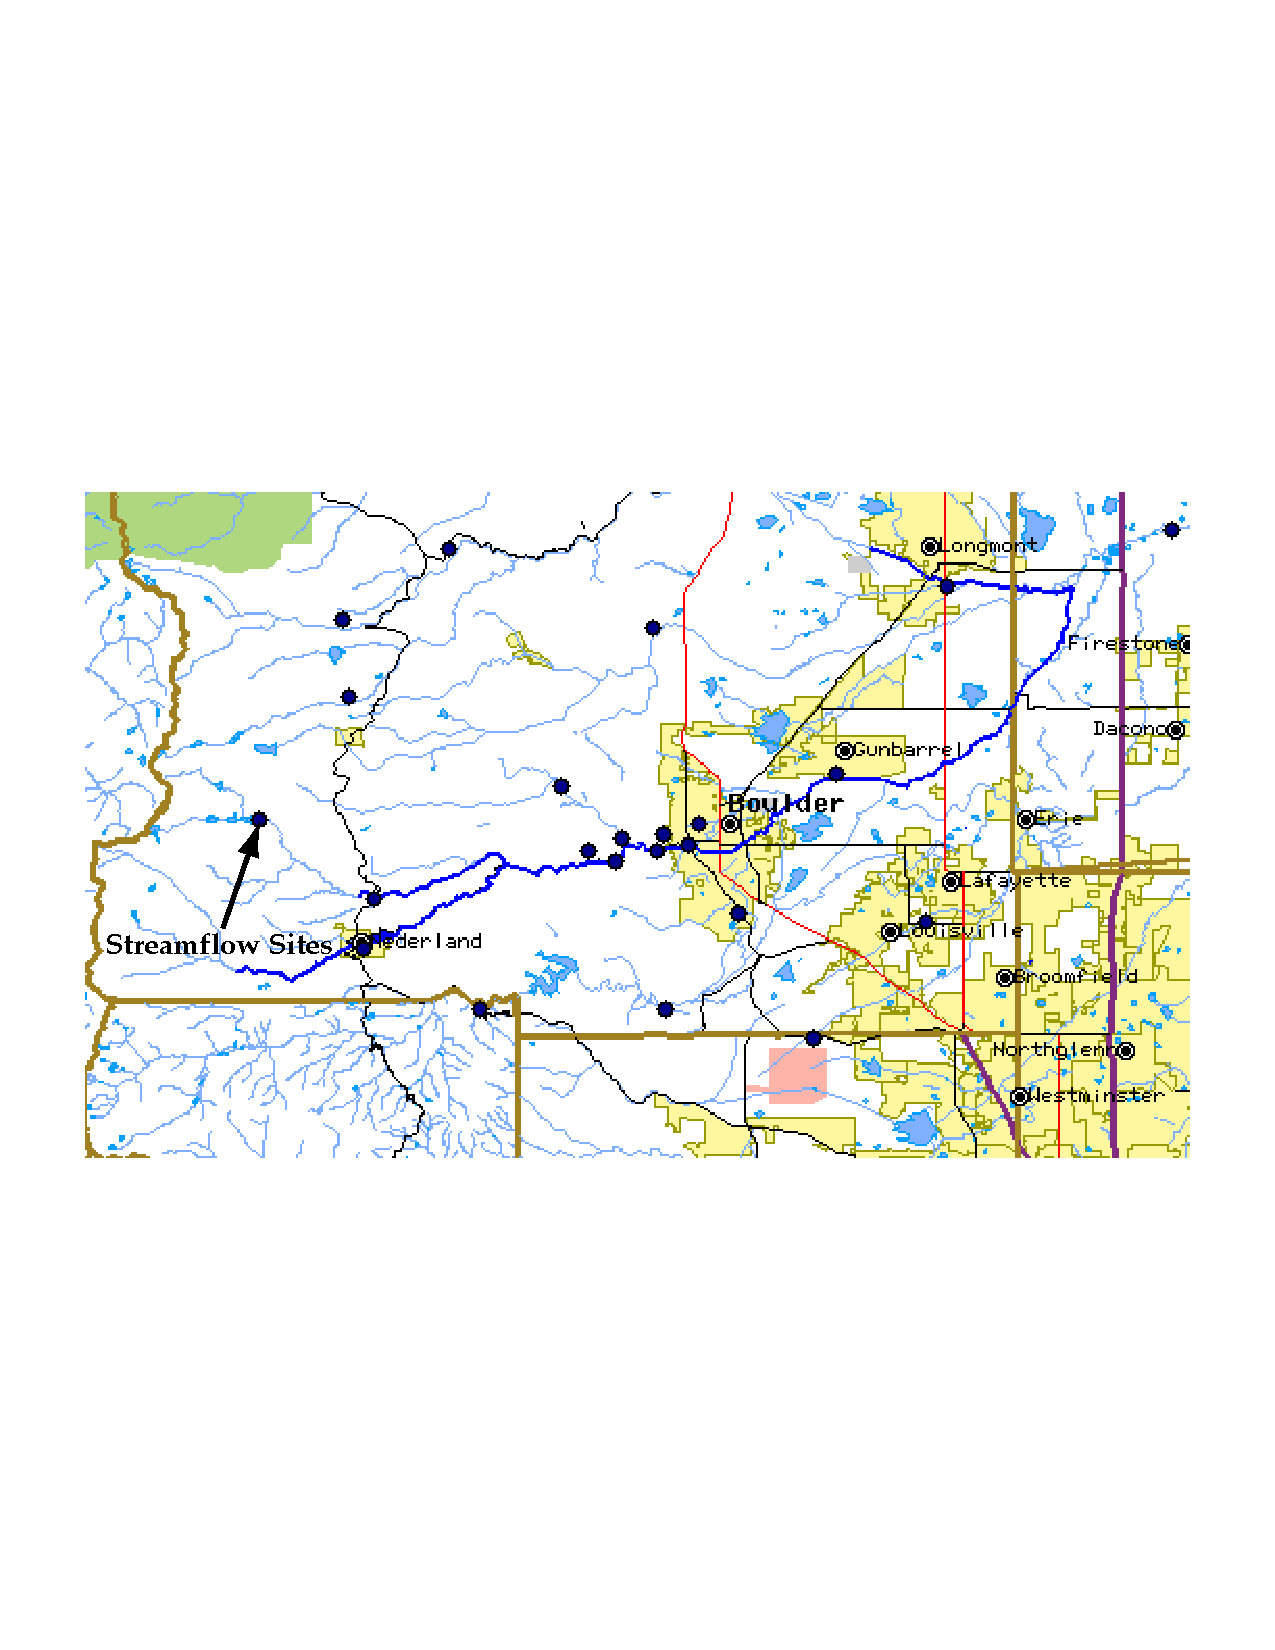
\includegraphics[width=.9\textwidth]{STREAMFLOW.pdf} 
   \caption{Boulder Creek Watershed Stream Flow Monitoring Sites (source: \url{http://bcn.boulder.co.us/basin/data/STREAMFLOW/STREAMFLOW.html})}
\end{figure}

\begin{figure}[htbp] %  figure placement: here, top, bottom, or page
   \centering
   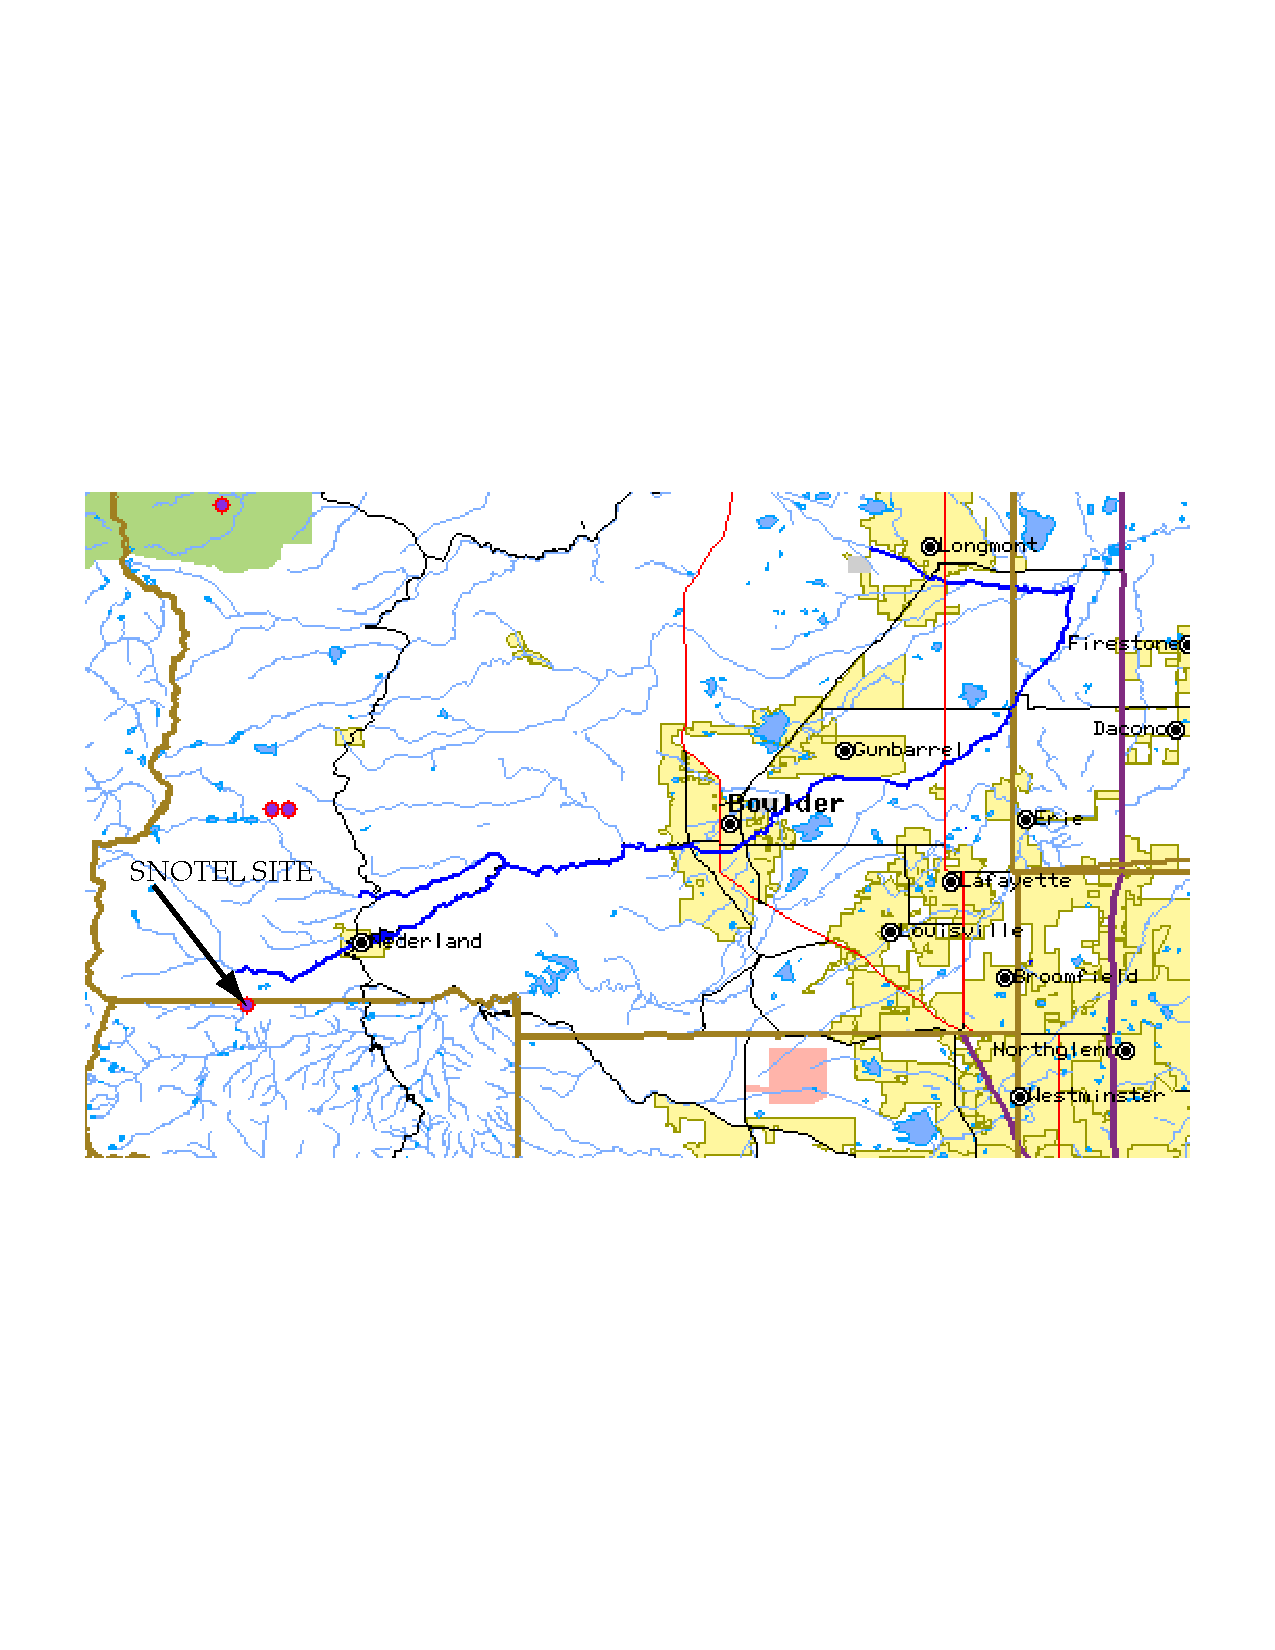
\includegraphics[width=.9\textwidth]{SNOTEL.pdf} 
   \caption{Boulder Creek Watershed Snowtel Snow Pack Monitoring (source: \url{http://bcn.boulder.co.us/basin/data/SNOTEL/SNOTEL.html})}
\end{figure}

\end{document}  